\documentclass[preprint,12pt]{elsarticle}

\journal{SoftwareX}

\usepackage{amsmath}
\usepackage{booktabs}
\usepackage{graphicx}
\usepackage{array}
\usepackage{xurl}
\Urlmuskip=0mu\relax
\usepackage[hidelinks]{hyperref}
\makeatletter
\newcommand{\metaurl}[1]{\href{#1}{\ttfamily\metaurl@break#1/\@nil}}
\def\metaurl@break#1/#2\@nil{%
  #1%
  \if\relax\detokenize{#2}\relax\else
    /\if\relax\detokenize{#1}\relax\else\allowbreak\fi
    \metaurl@break#2\@nil
  \fi
}
\makeatother
\usepackage{lineno}
\linenumbers

\graphicspath{{results/}}

\begin{document}

\begin{frontmatter}

\title{causalgeo: channel effects from concurrent geo holdouts}

\author[aff1]{Aditya Puttaparthi Tirumala\corref{cor1}}
\ead{puttaparthy.aditya@gmail.com}
\cortext[cor1]{Corresponding author.}
\address[aff1]{Independent Researcher}

\begin{abstract}
Marketing teams often run geo holdouts by turning off several media channels in different groups of markets at the same time. These experiments measure the incremental effect of each channel bundle, but standard geo-experiment tools do not separate the channels within a bundle, while marketing-mix models can produce unstable channel estimates when impressions move together.

\texttt{causalgeo} is a Python package for this setting. It assigns stratified concurrent cells, estimates each bundle effect from randomized holdout indicators, and checks whether the intervention schedule and delivered-impression paths can support a channel-level split. It fits linear channel slopes softly calibrated to the experimental bundle totals, reports the remaining model--experiment gap, and withholds slopes for channels that cannot be separated. On published geo impression paths with simulated outcomes of known slopes, the illustrative recovery is within 0.21 percent of the planted values. Across 200 draws per setting, the median absolute error runs from 0.20 percent for distinct paths to 2.24 percent for the channel that remains when a copied pair is withheld and the slopes are a quarter of the original size.
\end{abstract}

\begin{keyword}
geo experiment \sep incrementality \sep holdout \sep marketing mix \sep Python
\end{keyword}

\end{frontmatter}

\begin{table}[t]
\centering
\caption{Code metadata.}
\label{tab:metadata}
\setlength{\tabcolsep}{4pt}
\begin{tabular}{|l|>{\raggedright\arraybackslash}p{5.2cm}|>{\raggedright\arraybackslash}p{6.15cm}|}
\hline
\textbf{Nr.} & \textbf{Code metadata description} & \textbf{Value} \\
\hline
C1 & Current code version & 0.1.0 \\
\hline
C2 & Permanent link to code/repository used for this code version & \metaurl{https://github.com/adityapt/causalgeo/releases/tag/v0.1.0} \\
\hline
C3 & Permanent link to Reproducible Capsule & \metaurl{https://github.com/adityapt/causalgeo/blob/v0.1.0/paper/reproduce.py} \\
\hline
C4 & Legal Code License & MIT \\
\hline
C5 & Code versioning system used & git \\
\hline
C6 & Software code languages, tools, and services used & Python \\
\hline
C7 & Compilation requirements, operating environments and dependencies & Python $\geq$ 3.10. Runtime dependencies: pandas, numpy, scipy, statsmodels. The example also uses matplotlib. \\
\hline
C8 & Link to developer documentation & \metaurl{https://github.com/adityapt/causalgeo/blob/main/README.md} \\
\hline
C9 & Support email for questions & puttaparthy.aditya@gmail.com \\
\hline
\end{tabular}
\end{table}

\section{Motivation and significance}
\label{sec:motivation}

Geo experiments randomly change media in some markets and compare their outcome with unchanged markets \cite{vaver2011}. This avoids the selection bias in exposed-versus-unexposed comparisons \cite{lewis2011,gordon2019} and answers the practical question posed by a clean media off-switch: did the channel create incremental sales? \cite{blake2015}.

The limiting resource is usually the number of markets that can go dark. Consider a United States campaign spanning 210 designated market areas (DMAs). A business may permit a pause in only, say, 30 DMAs because large markets carry revenue risk, some regions have retailer or partner commitments, and others are reserved for ongoing campaigns. Those constraints determine the feasible holdout pool before an analyst can optimize geographic balance or power. Because advertising effects are small relative to sales noise \cite{lewisrao2015}, a powered single-channel holdout can exhaust that pool. Teams therefore turn off several channels in several cells during the same weeks. Each cell identifies its bundle effect, but not the effects of the channels within it.

Existing open tools address the single-cell problem: GeoLift selects markets and estimates lift with synthetic-control methods, while Meridian GeoX searches stratified designs and supports time-based regression, synthetic control, and synthetic difference-in-differences \cite{geolift,xu2017,geox2026,kerman2017,arkhangelsky2021}. They do not treat cells as channel bundles or reconcile a channel model with experimentally measured bundle totals. Conventional marketing-mix models can provide channel slopes from impression histories, but collinear media makes the split arbitrary \cite{chanperry2017,jin2017}. Bayesian marketing-mix models can regularize or calibrate channel slopes with experiment-derived priors, but a prior does not create a channel contrast absent from the experiment or the exposure paths; under nonidentification, the channel split remains prior-sensitive.

\texttt{causalgeo} is for this intermediate case. It estimates the experimentally identified bundle effect from the holdout indicator, then uses it as a weighted calibration row in a linear impression model. The resulting channel slopes are model-assisted, not direct experimental estimates. When the design or impression paths cannot distinguish a channel, the package reports the bundle rather than a fabricated channel value. Spend during the test is not used as a treatment regressor because it follows assignment \cite{angrist2009}.

\section{Software description}
\label{sec:software}

\subsection{Software architecture}
\label{sec:architecture}

The concurrent path, exposed through \texttt{design\_concurrent\_test} and \texttt{disentangle}, has four components.

\begin{enumerate}
\item \texttt{design.py} draws markets inside strata, builds the cell-by-channel schedule, and reports whether each channel is separate, tied, not tested, or not separable.
\item \texttt{identified.py} fits one holdout indicator per cell and withholds a channel coefficient unless a single cell turns that channel off alone.
\item \texttt{exposure.py} checks channels that were supposed to stay on. A shift that is large relative to the bundle effect is added as a covariate and the cell is refit.
\item \texttt{calibrated.py} fits a linear impression model on the pre-test weeks and on the control markets during the test, and adds one calibration equation per cell.
\end{enumerate}

The cell regression is a two-way within estimator with market-clustered standard errors \cite{wooldridge2010,bertrand2004,cameron2015}. The supporting \texttt{analyze} entry point also offers time-based regression, synthetic control, and synthetic difference-in-differences for an already assigned single-cell test. Market selection and power search remain the responsibility of GeoLift and GeoX \cite{geolift,geox2026}.

\subsection{Software functionalities}
\label{sec:function}

\paragraph{Design}
The caller supplies markets, strata, channels, and the off-channel bundle for each cell. Within strata, \texttt{control\_share} stays on and the remaining markets are divided among cells. The schedule is an indicator matrix $A_{kc}=1$ when cell $k$ turns channel $c$ off. The separation report labels zero columns as ``not tested,'' identical columns as ``tied,'' independent columns as ``separate,'' and remaining dependencies as ``not separable.''

\paragraph{Bundle effect}
Let $D_{it}^{(k)}=1$ when market $i$ is assigned to cell $k$ and week $t$ is in the test window. The cell regression is
\begin{equation}
\label{eq:cell}
Y_{it} = \sum_{k} \tau_{k}\, D_{it}^{(k)} + \alpha_{i} + \gamma_{t} + \varepsilon_{it}.
\end{equation}
The coefficient $\tau_{k}$ is the cell's sales change, relative to its own history and common week shocks. It is reported as a channel effect only for a separate channel tested alone. Overlapping bundles may span the channel space, but they do not justify assigning a bundle coefficient to one of their members.

\paragraph{Still-on channels}
A channel left on in cell $k$ can still differ between the dark markets and the control. The impression shift is the difference in differences
\begin{equation}
\label{eq:shift}
S_{kc} = \big(\bar X_{c,k,\mathrm{post}} - \bar X_{c,k,\mathrm{pre}}\big) - \big(\bar X_{c,\mathrm{control},\mathrm{post}} - \bar X_{c,\mathrm{control},\mathrm{pre}}\big).
\end{equation}
A pre-test, two-way-demeaned slope $b_{c}$ values this shift. If $|b_c S_{kc}|$ exceeds 10 percent of $|\tau_{k}|$, the cell is refit against the control with the still-on impressions as covariates. Turned-off channels are never covariates: their absence is the treatment. This correction is appropriate for a pre-existing imbalance, not when the holdout itself redirected budget to a still-on channel.

\paragraph{Channel split}
Let $W_{kc}$ be the impressions of channel $c$ withheld in cell $k$,
\begin{equation}
\label{eq:withheld}
W_{kc} = \max(-S_{kc},\, 0)
\end{equation}
for channels that cell $k$ turned off; all other entries in that calibration row are zero. The calibration target is $\sum_{c} \beta_{c} W_{kc} = -\tau_{k}$. It is a weighted row, not an equality constraint, in a two-way-demeaned impression model fit to all pre-test observations and to control markets during the test. Dark-market weeks are excluded. Observational rows use residual-variance weights; calibration rows use $1/\mathrm{se}(\tau_{k})^{2}$, so precise bundle estimates exert more influence. The bundle table reports any remaining gap.

The reported covariance is the inverse weighted cross-product. Bundle-target covariance is approximated as diagonal; shared controls and reuse of observational rows are therefore not fully modeled. The simulation assesses this approximation for the example design, not every possible panel.

Columns with cosine similarity above $1-10^{-6}$ are treated as copies. One remains as a shared control so its sales contribution is not pushed into the remaining channels, but neither receives a reported slope. Remaining columns pass a rank check. Daily impact is exposure times $\hat\beta_{c}$. Optional geometric adstock is available; saturation is deliberately absent because a single on/off holdout does not trace a response curve \cite{hanssens2001,jin2017}.

The returned tables are the channel slopes, the measured bundle effect next to the effect implied by $\hat\beta$ and $W_{kc}$, the exposure check, and the daily impacts.

\section{Illustrative examples}
\label{sec:example}

No public geo holdout ships with known channel-level effects. The example uses the published Meridian geo impression file \texttt{geo\_all\_channels.csv}: 40 markets and 156 weeks, from 25 January 2021 through 15 January 2024 \cite{meridiandata}. Sales are constructed so the slopes are known. Meridian's conversions column is used only to form strata. It is not the outcome, because that series already contains Meridian's own media response.

Three of the five channels are used, with planted slopes $2\times 10^{-4}$, $5\times 10^{-4}$, and $1\times 10^{-4}$ sales per impression. Strata are quartiles of each market's mean conversions. With \texttt{control\_share = 0.4} and seed 1, the design places 16 markets in control and 8 in each cell. The test window is the last 16 weeks, beginning 2 October 2023. In a dark market-week the turned-off channel's impressions are set to zero, and sales are
\begin{equation}
\label{eq:sales}
Y_{it} = \alpha_{i} + \gamma_{t} + \sum_{c} \beta_{c} X_{itc} + \varepsilon_{it},
\end{equation}
with $\alpha_{i}\sim N(0,50^{2})$, $\gamma_{t}\sim N(0,20^{2})$, and $\varepsilon_{it}\sim N(0,30^{2})$, drawn with seed 7. The script is \texttt{paper/example.py}.

The cells turn off $\{$Channel0, Channel1$\}$, $\{$Channel0, Channel2$\}$, and $\{$Channel1, Channel2$\}$, yielding rows $(1,1,0)$, $(1,0,1)$, and $(0,1,1)$. The schedule has full column rank, but no channel is tested alone; the assignment-only table therefore leaves all three channel effects blank. Table~\ref{tab:slopes} instead reports the impression-model slopes, softly calibrated to the three measured bundles.

This is a recovery check for the linear model that the package fits, not evidence about saturation, long carryover, or the power of an eight-market cell. The impression paths are external to the package; sales are constructed from known slopes. Real experiments with smaller effects will have wider intervals \cite{lewisrao2015}.

\begin{table}[t]
\centering
\caption{Cell effects on the constructed series. The adjusted column replaces the cell coefficient when a still-on channel's sales-valued shift exceeds 10 percent of the unadjusted effect. The model column values the same impression change at the fitted slopes: the difference-in-differences in impressions for the channels that cell turned off.}
\label{tab:cells}
\begin{tabular}{llrrrr}
\toprule
Cell & Bundle & Unadjusted & Adjusted & SE & Model \\
\midrule
1 & Channel0+Channel1 & $-555.7$ & $-587.2$ & 71.4 & $-570.2$ \\
2 & Channel0+Channel2 & $-318.0$ & $-251.5$ & 36.2 & $-253.6$ \\
3 & Channel1+Channel2 & $-399.9$ & $-399.9$ & 54.4 & $-396.2$ \\
\bottomrule
\end{tabular}
\end{table}

\begin{figure}[t]
\centering
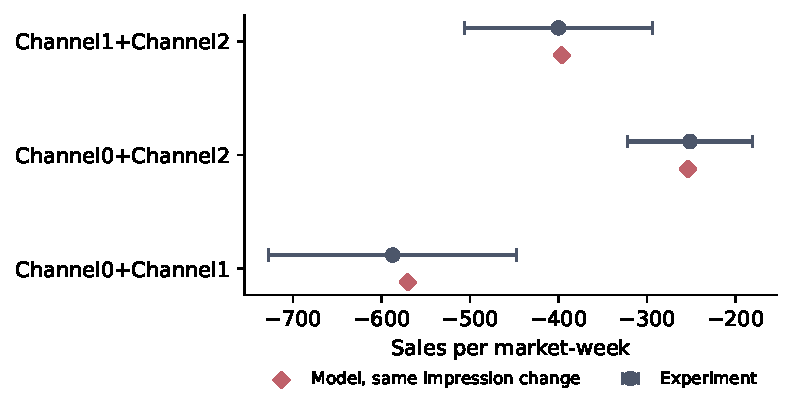
\includegraphics[width=0.92\linewidth]{bundle_contrast.pdf}
\caption{Experimental bundle effect, with a 95 percent interval, and the same off-channel impression change valued at the fitted slopes. Sales per market-week.}
\label{fig:bundles}
\end{figure}

Cell 2 illustrates the exposure correction: Channel1's still-on shift is worth $-83$ sales, or 26 percent of the unadjusted effect, and refitting moves the estimate from $-318.0$ to $-251.5$. The corresponding shares are 13 percent for Cell 1 and 0.5 percent for Cell 3.

\begin{table}[t]
\centering
\caption{Planted and recovered slopes, in sales per 10{,}000 impressions. The largest absolute error is 0.21 percent.}
\label{tab:slopes}
\begin{tabular}{lrrrr}
\toprule
Channel & Planted & Recovered & SE & Abs. error (\%) \\
\midrule
Channel0 & 2.000 & 1.997 & 0.006 & 0.17 \\
Channel1 & 5.000 & 5.009 & 0.008 & 0.17 \\
Channel2 & 1.000 & 1.002 & 0.008 & 0.21 \\
\bottomrule
\end{tabular}
\end{table}

\begin{table}[t]
\centering
\caption{Two hundred refits per setting. Rho is the weight on Channel0 in the untreated Channel1 path. Error is the median absolute percent error among reported slopes. Coverage is the mean within-run coverage; brackets give its 95 percent Monte Carlo interval. At rho 1, error and coverage refer to the remaining channel.}
\label{tab:reliability}
\small
\setlength{\tabcolsep}{4pt}
\begin{tabular}{rrrrlr}
\toprule
Scale & Rho & Runs & Median error (\%) & Coverage [MC interval] & Pair withheld \\
\midrule
1.00 & 0.0 & 200 & 0.20 & 0.958 [0.942, 0.974] & 0.00 \\
1.00 & 0.9 & 200 & 0.40 & 0.953 [0.934, 0.973] & 0.00 \\
1.00 & 1.0 & 200 & 0.58 & 0.940 [0.907, 0.973] & 1.00 \\
0.25 & 0.0 & 200 & 0.77 & 0.958 [0.942, 0.974] & 0.00 \\
0.25 & 0.9 & 200 & 1.63 & 0.957 [0.938, 0.975] & 0.00 \\
0.25 & 1.0 & 200 & 2.24 & 0.940 [0.907, 0.973] & 1.00 \\
\bottomrule
\end{tabular}
\end{table}

Table~\ref{tab:cells} compares experimental and model-implied bundle effects. Their gaps are 2.9, 0.8, and 0.9 percent of the experimental effects; all model totals lie within the experimental intervals. The bundle coefficient remains the experimental result, while the channel slope is the model-assisted split.

When Channel1 is replaced with a copy of Channel0, both are withheld. Their shared path remains as one control: Channel2 is then recovered as 0.97 sales per 10{,}000 impressions, versus its planted 1.00. Omitting the shared path instead biases it to 3.02.

Table~\ref{tab:reliability} and Figure~\ref{fig:separation} summarize 200 noise draws for each slope scale and degree of Channel0--Channel1 similarity. At the original scale, median absolute error is 0.20 percent for distinct paths and 0.40 percent at a 0.9 mix; coverage is 95.8 and 95.3 percent. At an exact copy, the pair is withheld in every run and the remaining channel covers in 94.0 percent of runs (95 percent Monte Carlo interval: 90.7--97.3 percent). These results assess this design and the diagonal covariance approximation; they are not a general guarantee.

\begin{figure}[t]
\centering
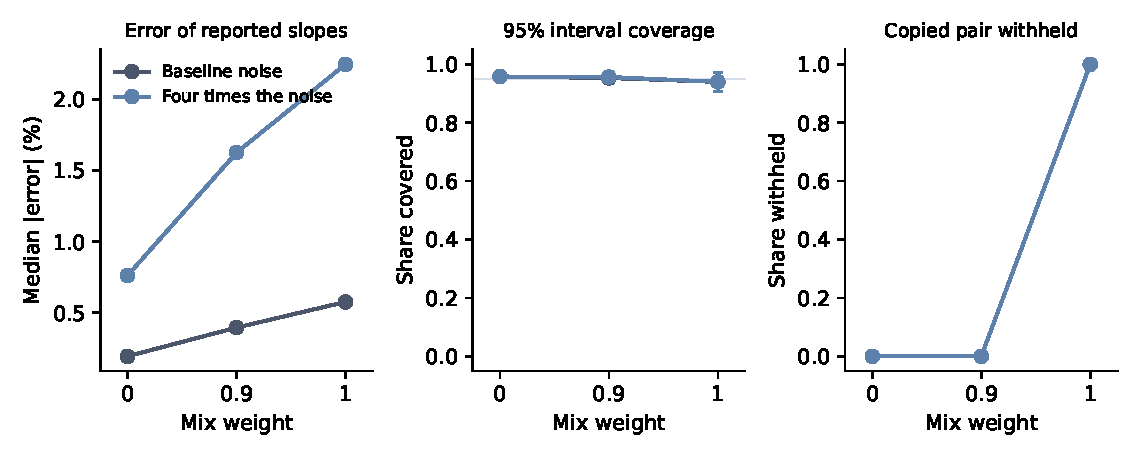
\includegraphics[width=\linewidth]{separation.pdf}
\caption{Recovery over 200 simulations per setting as the untreated Channel1 path is mixed toward Channel0. Bars in the coverage panel are 95 percent Monte Carlo intervals. At mix weight 1 the pair is withheld in every run, so error and coverage refer to the remaining channel.}
\label{fig:separation}
\end{figure}

\section{Impact}
\label{sec:impact}

The package gives a team that must test channels in bundles one place to assign the cells, see which channels the design can name, read the bundle effects from the holdout indicators, and produce channel slopes with the remaining gap reported next to those effects. Existing open geo libraries stop at the cell \cite{geolift,geox2026}. Analysts who need a channel number have had to do the split in a separate mix model \cite{chanperry2017,jin2017}, with no report of how far the split sits from the experimental total, and no refusal when two channels moved together. The same separation of a fine estimand from a coarse one is what recent panel software has started to make explicit \cite{clark2025}. Here the coarse object is the bundle, and the fine object is the channel.

The current release is 0.1.0. Adoption is early, and this paper does not report a user study. The reusable piece is the example: \texttt{paper/reproduce.py} rebuilds Tables~\ref{tab:cells}, \ref{tab:slopes}, and \ref{tab:reliability}, and both figures. The same functions apply to a real holdout once the caller supplies the market outcome and the channel impressions. Channels the design cannot separate, and channels whose impressions are copies, stay blank, which is the output a downstream budget decision can tell from a slope that was actually estimated.

\section{Conclusions}
\label{sec:conclusions}

\texttt{causalgeo} measures concurrent channel-bundle holdouts and splits each measured total into channel slopes when the impression histories support the split. The calibration is soft and uses the experiment's pre/post impression contrast. On the published Meridian paths the three slopes are recovered to within 0.21 percent, and their bundle totals are 0.8 to 2.9 percent from the experimental effects. A copied pair is controlled for as one path and is not split. Across 200 simulations per setting, the channel that remains is close to its planted slope and its nominal interval covers in 94 percent of runs. Coverage across the six settings ranges from 94.0 to 95.8 percent, with Monte Carlo intervals that include 95 percent. These intervals remain conditional on the fitted linear model and the diagonal approximation for estimated bundle targets.

The split is linear, with an optional geometric adstock and no saturation curve \cite{jin2017}. A holdout that switches a channel off does not trace the curve between those two points, so the package does not estimate one. Market-selection and power search are left to GeoLift and GeoX \cite{geolift,geox2026}; this package assigns markets inside strata the caller already chose, and it does not claim that eight markets are a powered cell \cite{lewisrao2015}. The still-on adjustment should be read against the design of the test: it removes a pre-existing impression imbalance, and it should be turned off when the holdout itself is what moved the budget. Spend during the test stays out of the regression, because it is a result of the assignment rather than a confounder of it \cite{angrist2009,lewis2011}.

\section*{CRediT authorship contribution statement}
Aditya Puttaparthi Tirumala: Conceptualization, Methodology, Software, Validation, Writing -- original draft, Writing -- review and editing.

\section*{Declaration of competing interest}
The author declares that he has no known competing financial interests or personal relationships that could have appeared to influence the work reported in this paper.

\section*{Data availability}
The impression paths are the Meridian file \texttt{geo\_all\_channels.csv} \cite{meridiandata}. In \texttt{paper/}, set \texttt{PYTHONPATH=../src} and run \texttt{python3.11 reproduce.py}. That rebuilds Tables~\ref{tab:cells}, \ref{tab:slopes}, and \ref{tab:reliability} and both figures, then checks them against the rounded values reported here. Table~\ref{tab:metadata} gives the repository links.

\section*{Declaration of generative AI and AI-assisted technologies in the manuscript preparation process}
During the preparation of this work the author used Cursor, with the Grok language model, to draft and revise the manuscript and the example code. After using this tool, the author reviewed and edited the content as needed and takes full responsibility for the content of the published article.

\bibliographystyle{elsarticle-num}
\bibliography{references}

\end{document}
